% Options for packages loaded elsewhere
\PassOptionsToPackage{unicode}{hyperref}
\PassOptionsToPackage{hyphens}{url}
%
\documentclass[
  ignorenonframetext,
  aspectratio=169,
]{beamer}
\usepackage{pgfpages}
\setbeamertemplate{caption}[numbered]
\setbeamertemplate{caption label separator}{: }
\setbeamercolor{caption name}{fg=normal text.fg}
\beamertemplatenavigationsymbolsempty
% Prevent slide breaks in the middle of a paragraph
\widowpenalties 1 10000
\raggedbottom
\setbeamertemplate{part page}{
  \centering
  \begin{beamercolorbox}[sep=16pt,center]{part title}
    \usebeamerfont{part title}\insertpart\par
  \end{beamercolorbox}
}
\setbeamertemplate{section page}{
  \centering
  \begin{beamercolorbox}[sep=12pt,center]{part title}
    \usebeamerfont{section title}\insertsection\par
  \end{beamercolorbox}
}
\setbeamertemplate{subsection page}{
  \centering
  \begin{beamercolorbox}[sep=8pt,center]{part title}
    \usebeamerfont{subsection title}\insertsubsection\par
  \end{beamercolorbox}
}
\AtBeginPart{
  \frame{\partpage}
}
\AtBeginSection{
  \ifbibliography
  \else
    \frame{\sectionpage}
  \fi
}
\AtBeginSubsection{
  \frame{\subsectionpage}
}

\usepackage{amsmath,amssymb}
\usepackage{iftex}
\ifPDFTeX
  \usepackage[T1]{fontenc}
  \usepackage[utf8]{inputenc}
  \usepackage{textcomp} % provide euro and other symbols
\else % if luatex or xetex
  \usepackage{unicode-math}
  \defaultfontfeatures{Scale=MatchLowercase}
  \defaultfontfeatures[\rmfamily]{Ligatures=TeX,Scale=1}
\fi
\usepackage{lmodern}
\usetheme[progressbar=frametitle]{moloch}
\ifPDFTeX\else  
    % xetex/luatex font selection
\fi
% Use upquote if available, for straight quotes in verbatim environments
\IfFileExists{upquote.sty}{\usepackage{upquote}}{}
\IfFileExists{microtype.sty}{% use microtype if available
  \usepackage[]{microtype}
  \UseMicrotypeSet[protrusion]{basicmath} % disable protrusion for tt fonts
}{}
\makeatletter
\@ifundefined{KOMAClassName}{% if non-KOMA class
  \IfFileExists{parskip.sty}{%
    \usepackage{parskip}
  }{% else
    \setlength{\parindent}{0pt}
    \setlength{\parskip}{6pt plus 2pt minus 1pt}}
}{% if KOMA class
  \KOMAoptions{parskip=half}}
\makeatother
\usepackage{xcolor}
\newif\ifbibliography
\setlength{\emergencystretch}{3em} % prevent overfull lines
\setcounter{secnumdepth}{-\maxdimen} % remove section numbering


\providecommand{\tightlist}{%
  \setlength{\itemsep}{0pt}\setlength{\parskip}{0pt}}\usepackage{longtable,booktabs,array}
\usepackage{calc} % for calculating minipage widths
\usepackage{caption}
% Make caption package work with longtable
\makeatletter
\def\fnum@table{\tablename~\thetable}
\makeatother
\usepackage{graphicx}
\makeatletter
\def\maxwidth{\ifdim\Gin@nat@width>\linewidth\linewidth\else\Gin@nat@width\fi}
\def\maxheight{\ifdim\Gin@nat@height>\textheight\textheight\else\Gin@nat@height\fi}
\makeatother
% Scale images if necessary, so that they will not overflow the page
% margins by default, and it is still possible to overwrite the defaults
% using explicit options in \includegraphics[width, height, ...]{}
\setkeys{Gin}{width=\maxwidth,height=\maxheight,keepaspectratio}
% Set default figure placement to htbp
\makeatletter
\def\fps@figure{htbp}
\makeatother

\setbeamertemplate{caption}[default]
%\setbeamertemplate{caption name}{\raggedright\insertcaption\par}
\setbeamertemplate{caption label seperator}[none]
%\setbeamerfont{footnote}{size=\tiny}
\definecolor{twriBlue}{HTML}{0054a4}
\definecolor{spotMaroon}{HTML}{5d0025}
\setbeamercolor{alerted text}{fg=spotMaroon}
\setbeamercolor{frametitle}{bg=twriBlue}
\usepackage{fontspec}

\setsansfont{Open Sans}

% title logos
\titlegraphic{%
    
\includegraphics[width=.2\textwidth]{logo}\hfill
  
\includegraphics[width=.2\textwidth]{logo-AgriLife}\hfill
  
\includegraphics[width=.2\textwidth]{logo-TSSWCB}
}


\makeatletter
\setbeamertemplate{title page}{
  \begin{minipage}[b][\paperheight]{\textwidth}
    \vfill%
    \ifx\inserttitle\@empty\else\usebeamertemplate*{title}\fi
    \ifx\insertsubtitle\@empty\else\usebeamertemplate*{subtitle}\fi
    \usebeamertemplate*{title separator}
    \ifx\beamer@shortauthor\@empty\else\usebeamertemplate*{author}\fi
    \ifx\insertdate\@empty\else\usebeamertemplate*{date}\fi
    \ifx\insertinstitute\@empty\else\usebeamertemplate*{institute}\fi
    \vfill
    \ifx\inserttitlegraphic\@empty\else\inserttitlegraphic\fi
    \vspace*{1cm}
  \end{minipage}
}
\makeatother
\usepackage{booktabs}
\usepackage{longtable}
\usepackage{array}
\usepackage{multirow}
\usepackage{wrapfig}
\usepackage{float}
\usepackage{colortbl}
\usepackage{pdflscape}
\usepackage{tabu}
\usepackage{threeparttable}
\usepackage{threeparttablex}
\usepackage[normalem]{ulem}
\usepackage{makecell}
\usepackage{xcolor}
\makeatletter
\@ifpackageloaded{caption}{}{\usepackage{caption}}
\AtBeginDocument{%
\ifdefined\contentsname
  \renewcommand*\contentsname{Table of contents}
\else
  \newcommand\contentsname{Table of contents}
\fi
\ifdefined\listfigurename
  \renewcommand*\listfigurename{List of Figures}
\else
  \newcommand\listfigurename{List of Figures}
\fi
\ifdefined\listtablename
  \renewcommand*\listtablename{List of Tables}
\else
  \newcommand\listtablename{List of Tables}
\fi
\ifdefined\figurename
  \renewcommand*\figurename{Figure}
\else
  \newcommand\figurename{Figure}
\fi
\ifdefined\tablename
  \renewcommand*\tablename{Table}
\else
  \newcommand\tablename{Table}
\fi
}
\@ifpackageloaded{float}{}{\usepackage{float}}
\floatstyle{ruled}
\@ifundefined{c@chapter}{\newfloat{codelisting}{h}{lop}}{\newfloat{codelisting}{h}{lop}[chapter]}
\floatname{codelisting}{Listing}
\newcommand*\listoflistings{\listof{codelisting}{List of Listings}}
\makeatother
\makeatletter
\makeatother
\makeatletter
\@ifpackageloaded{caption}{}{\usepackage{caption}}
\@ifpackageloaded{subcaption}{}{\usepackage{subcaption}}
\makeatother

\ifLuaTeX
  \usepackage{selnolig}  % disable illegal ligatures
\fi
\usepackage[style=apa,]{biblatex}
\addbibresource{bibliography.bib}
\usepackage{bookmark}

\IfFileExists{xurl.sty}{\usepackage{xurl}}{} % add URL line breaks if available
\urlstyle{same} % disable monospaced font for URLs
\hypersetup{
  pdftitle={The Meta-Analysis of Nonpoint Source BMPs: Can We Improve the Empirical Knowledge Associated with BMP Water Quality Improvement?},
  pdfauthor={Michael Schramm, Duncan Kikoyo, Janelle Wright, Shubham Jain},
  hidelinks,
  pdfcreator={LaTeX via pandoc}}


\title{The Meta-Analysis of Nonpoint Source BMPs: Can We Improve the
Empirical Knowledge Associated with BMP Water Quality Improvement?}
\author{Michael Schramm, Duncan Kikoyo, Janelle Wright, Shubham Jain}
\date{2024-08-30}
\institute{Texas Water Resources Institute, Texas A\&M AgriLife
Research.\hfill \break Project funding provided by the Texas State Soil
and Water Conservation Board. \hfill \break 2024 AWRA, UCOWR, \& NIWR
Joint Water Resources Conference}

\begin{document}
\frame{\titlepage}




\begin{frame}{Introduction}
\phantomsection\label{introduction}
\begin{block}{Purpose}
\phantomsection\label{purpose}
\begin{itemize}
\tightlist
\item
  Assess scope and scale of published water quality BMP field studies.
\item
  Assess mean reductions in pollutant \emph{concentrations} in BMP
  studies.
\item
  Methods and results fully detailed in Frontiers article
  \footfullcite{schrammMetaanalysisImpactsBest2024}
\end{itemize}
\end{block}
\end{frame}

\begin{frame}{Methods}
\phantomsection\label{methods}
\begin{block}{Systematic Review}
\phantomsection\label{systematic-review}
\begin{itemize}
\item
  Followed systematic review guidance in Collaboration for Environmental
  Evidence
  \footfullcite{collaborationforenvironmentalevidenceGuidelinesStandardsEvidence2018}
\item
  Review identified \textbf{90 studies} and \textbf{642 effect sizes}
\item
  Collected data included: \emph{Publication date, measured parameters,
  runoff source, BMP type, study scale, location, study length,
  measurement units, control and treatment sample size, standard error,
  standard deviation, mean concentration, etc.}
\item
  Raw data available on Zenodo
  \footfullcite{kikoyoTWRINonpointSource2023}
\end{itemize}
\end{block}
\end{frame}

\begin{frame}{Methods}
\phantomsection\label{methods-1}
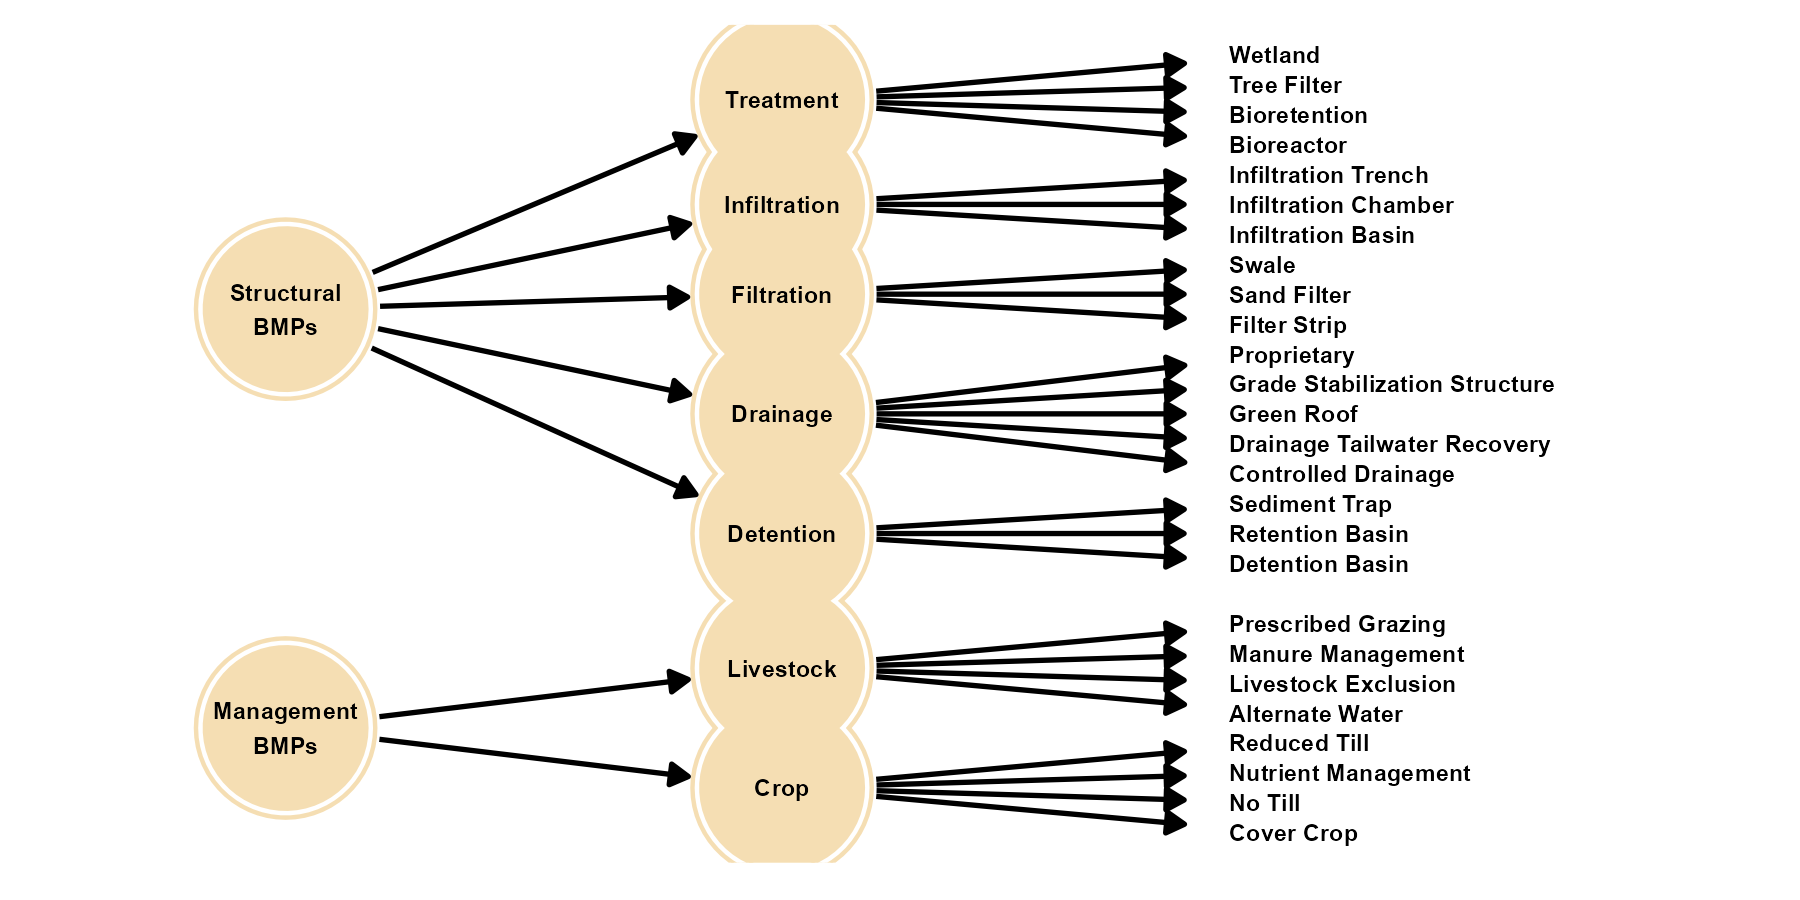
\includegraphics{Schramm-UCOWR-2024_files/figure-beamer/bmpstruct-1.png}
\end{frame}

\begin{frame}{Methods}
\phantomsection\label{methods-2}
\begin{block}{Meta-Analysis}
\phantomsection\label{meta-analysis}
\begin{itemize}
\tightlist
\item
  Describe overall effect and heterogeneity
\item
  Weighted multilevel random effects models

  \begin{itemize}
  \tightlist
  \item
    Weights individual effect sizes based on sampling variance
  \end{itemize}
\item
  Model terms:

  \begin{itemize}
  \tightlist
  \item
    Influent pollutant concentration
  \item
    BMP category
  \item
    Aridity index: \(\frac{\bar{P}}{\bar{PET}}\)
    \footfullcite{zomerVersionGlobalAridity2022}
  \item
    Fixed effect interactions
  \item
    Nested random effects \((Effect|Study)\)
  \end{itemize}
\end{itemize}
\end{block}
\end{frame}

\begin{frame}{Methods}
\phantomsection\label{methods-3}
\begin{block}{Meta-Analysis}
\phantomsection\label{meta-analysis-1}
\begin{itemize}
\tightlist
\item
  Dependent variable: log ratio of means
\end{itemize}

\[
ROM_i = ln(\frac{x_{i,control}}{x_{i,trmt}}) = ln(x_{i,control}) - ln(x_{i,trmt})
\] - Separate models for each parameter of interest: \textbf{fecal
indicator bacteria} (FIB), \textbf{total nitrogen} (TN), \textbf{total
phosphorus} (TP), \textbf{total suspended sediment} (TSS),
\textbf{orthophosphate} (PO\textsubscript{4}), \textbf{dissolved
inorganic nitrogen} (DIN).
\end{block}
\end{frame}

\begin{frame}{Study Scale \& Source}
\phantomsection\label{study-scale-source}
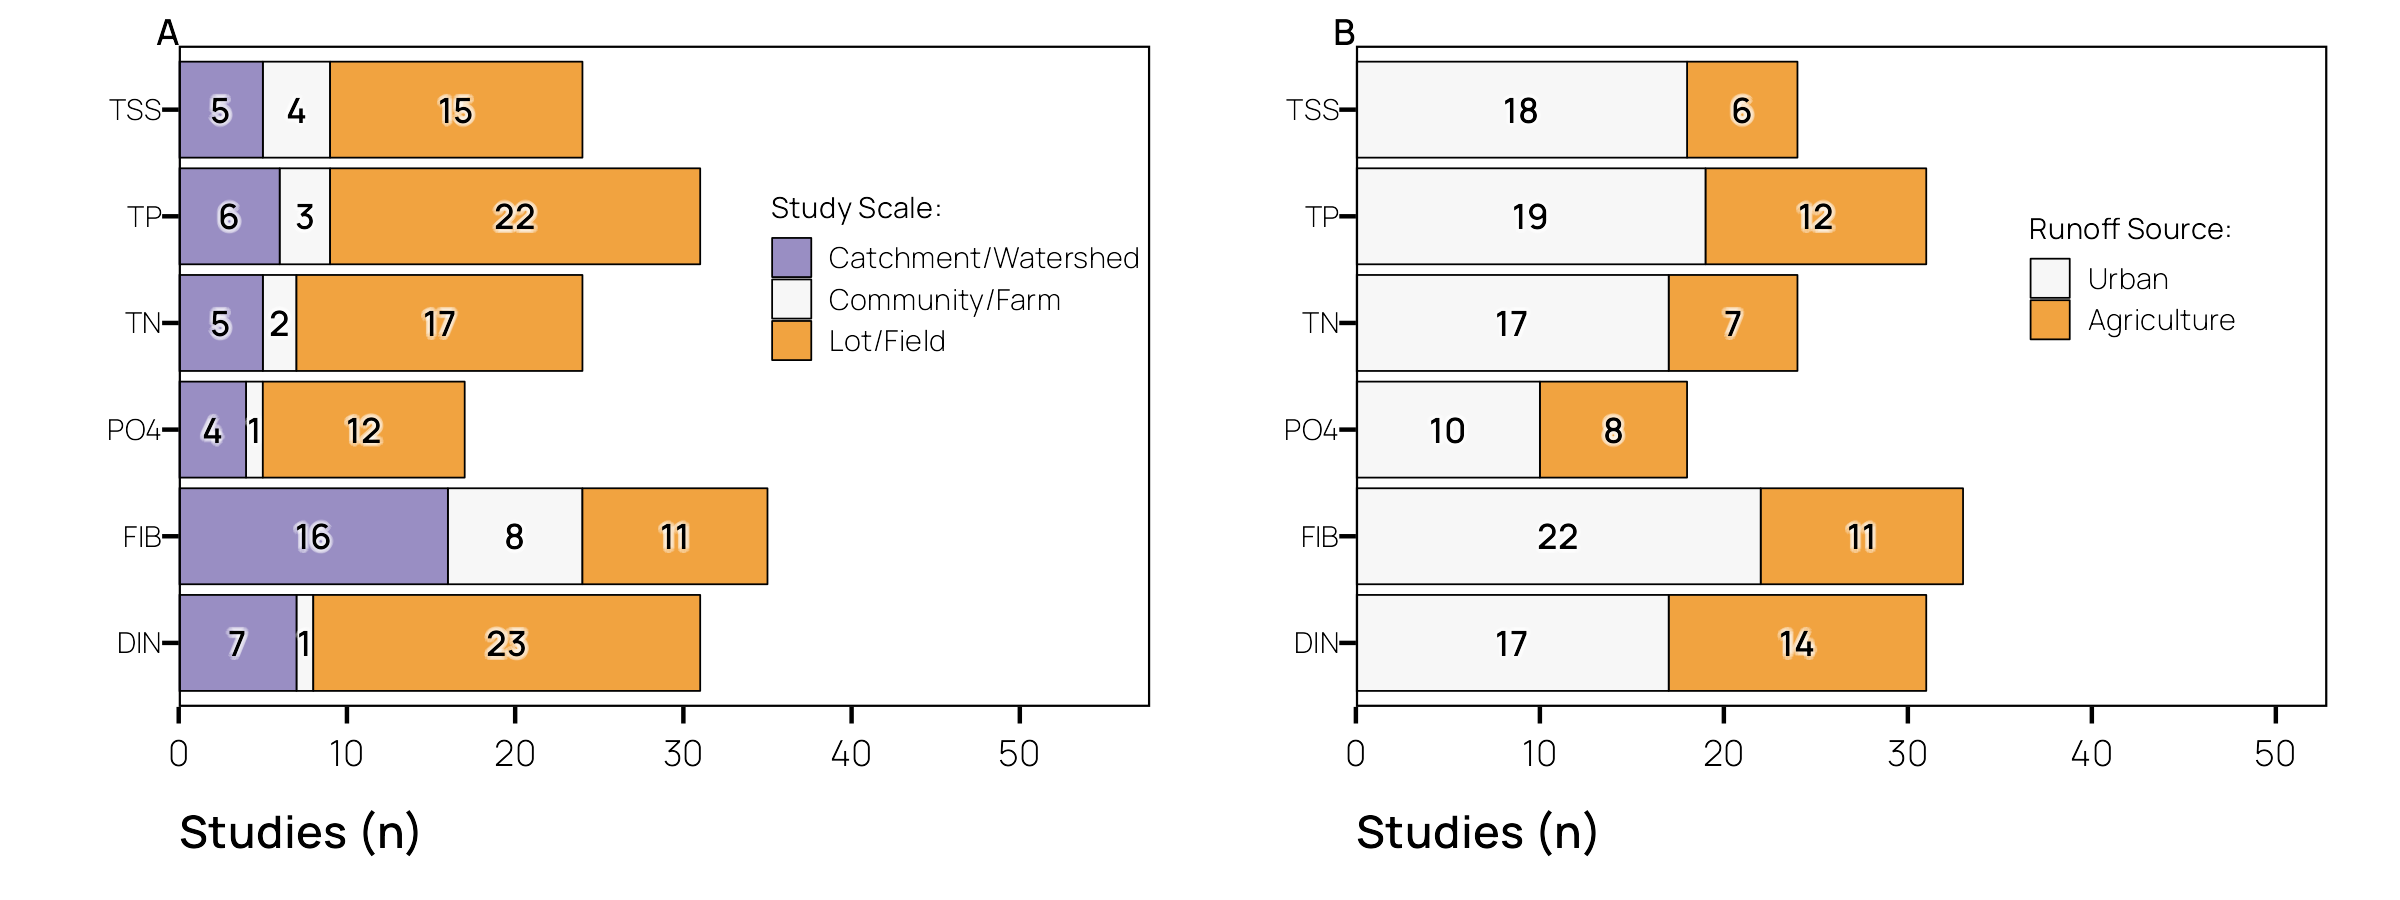
\includegraphics[width=1\textwidth,height=\textheight]{Schramm-UCOWR-2024_files/figure-beamer/p1-1.png}

\begin{itemize}
\tightlist
\item
  Most studies were lot/field scale and investigated urbanized runoff.
\item
  FIB studies tended toward larger catchments.
\end{itemize}
\end{frame}

\begin{frame}{Publication Date and Study Length}
\phantomsection\label{publication-date-and-study-length}
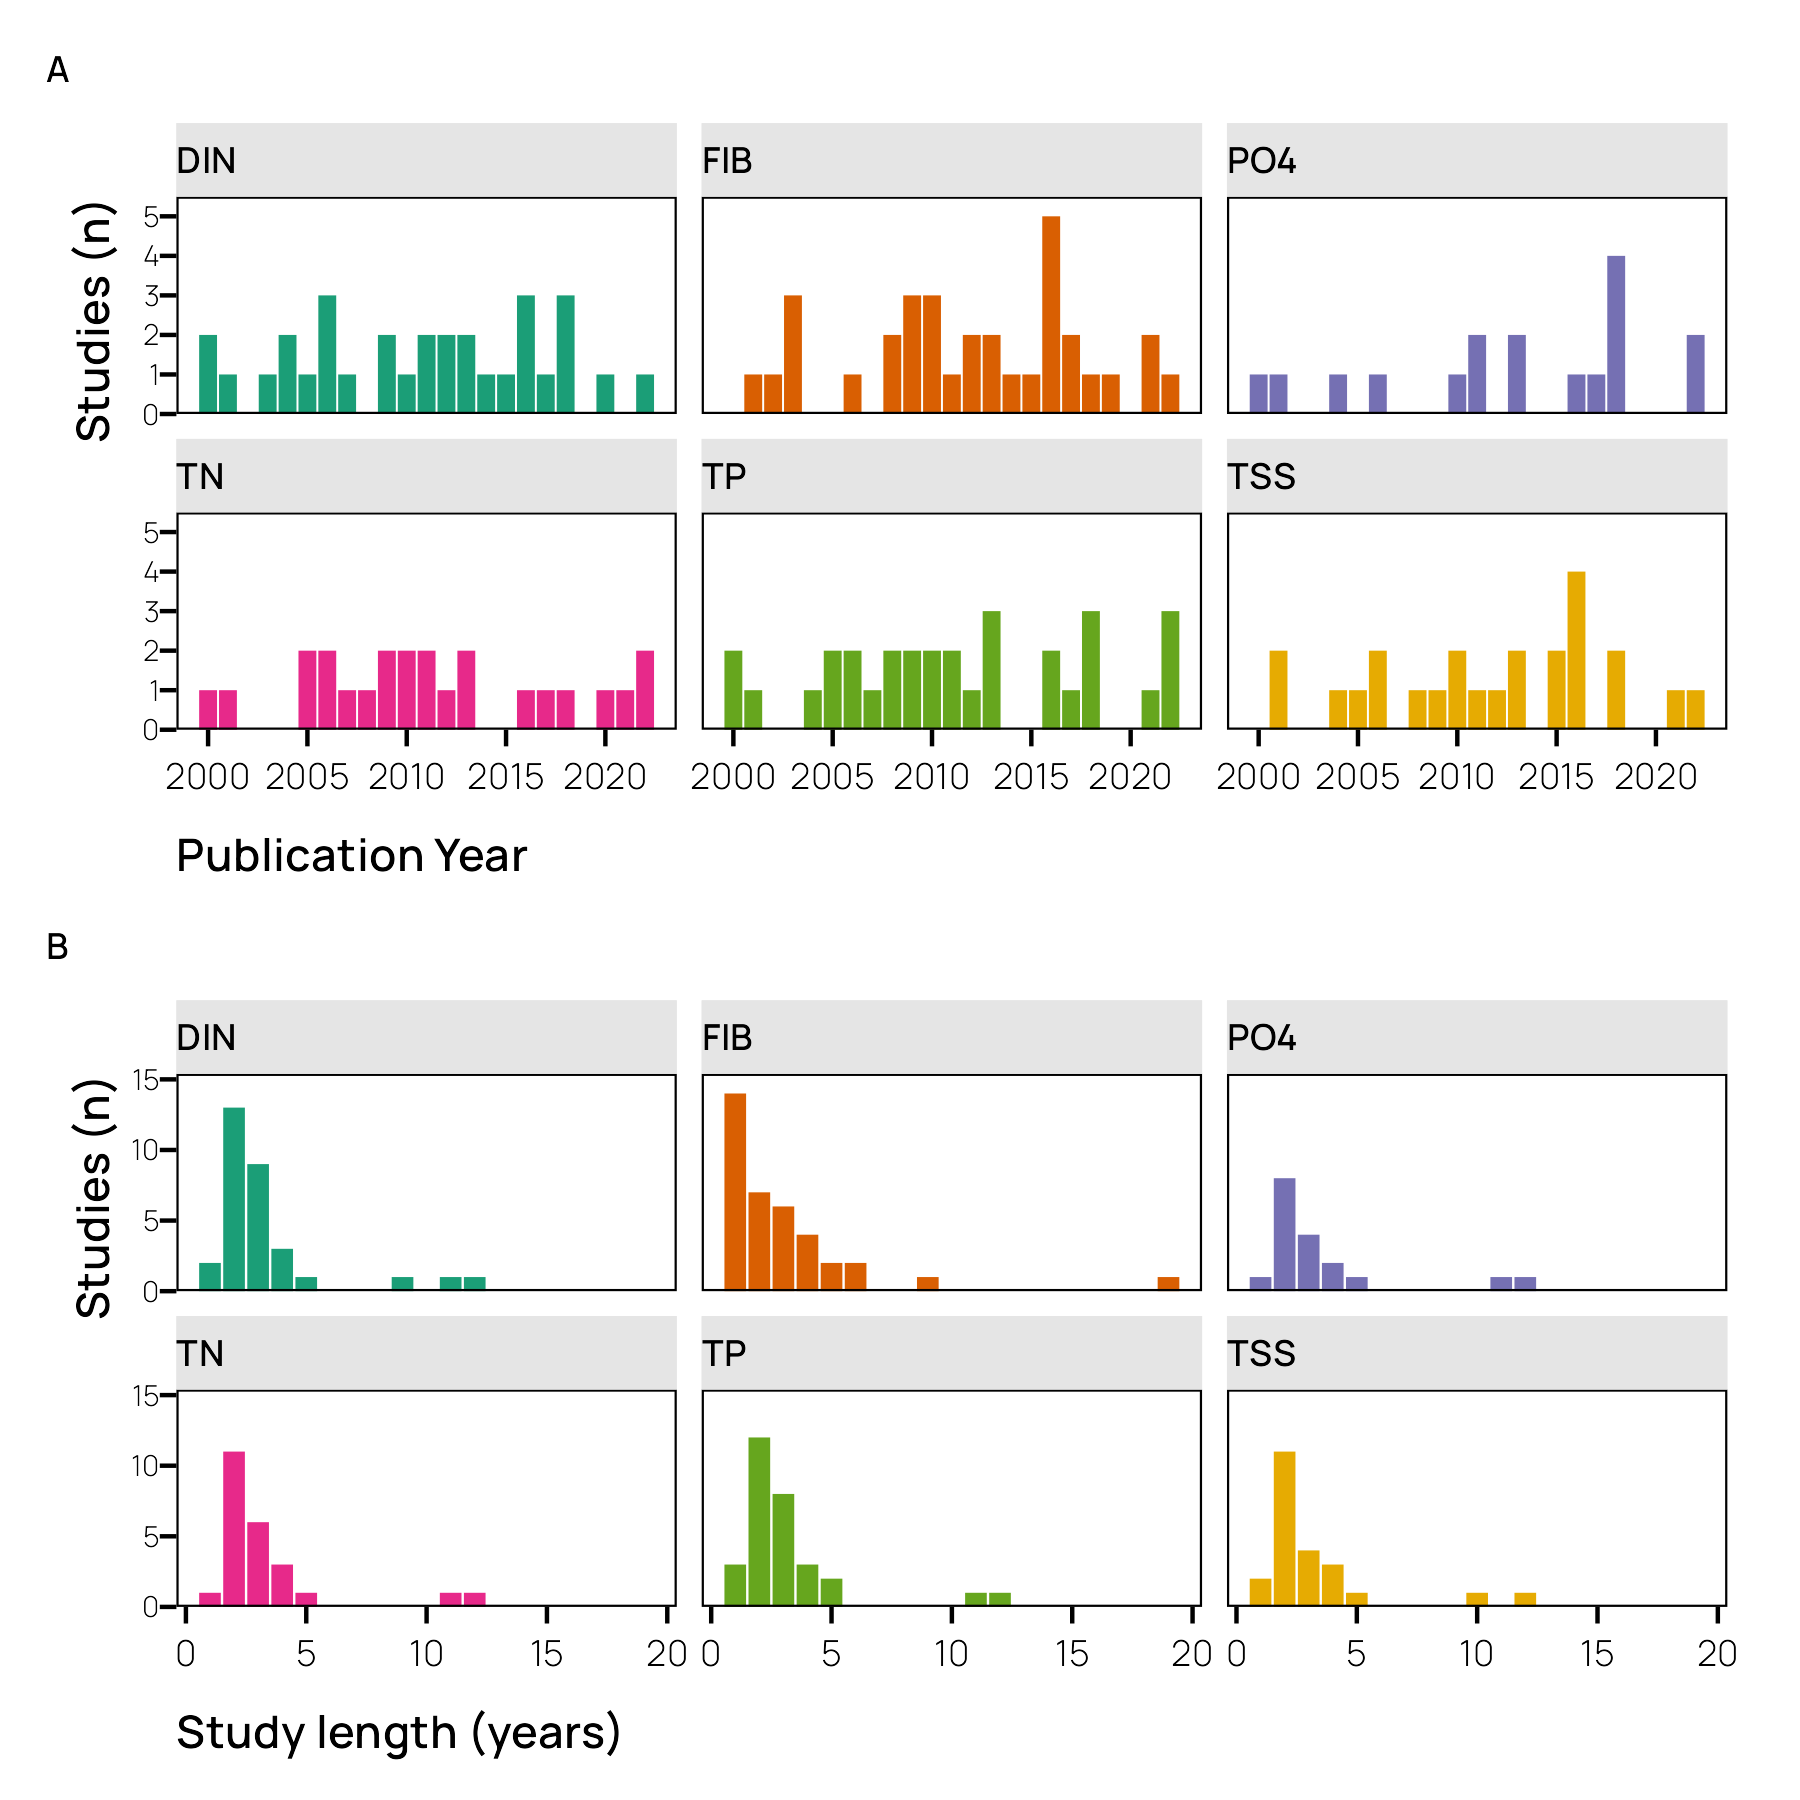
\includegraphics[width=0.5\textwidth,height=\textheight]{Schramm-UCOWR-2024_files/figure-beamer/p2-1.png}
\end{frame}

\begin{frame}{Spatial Distribution}
\phantomsection\label{spatial-distribution}
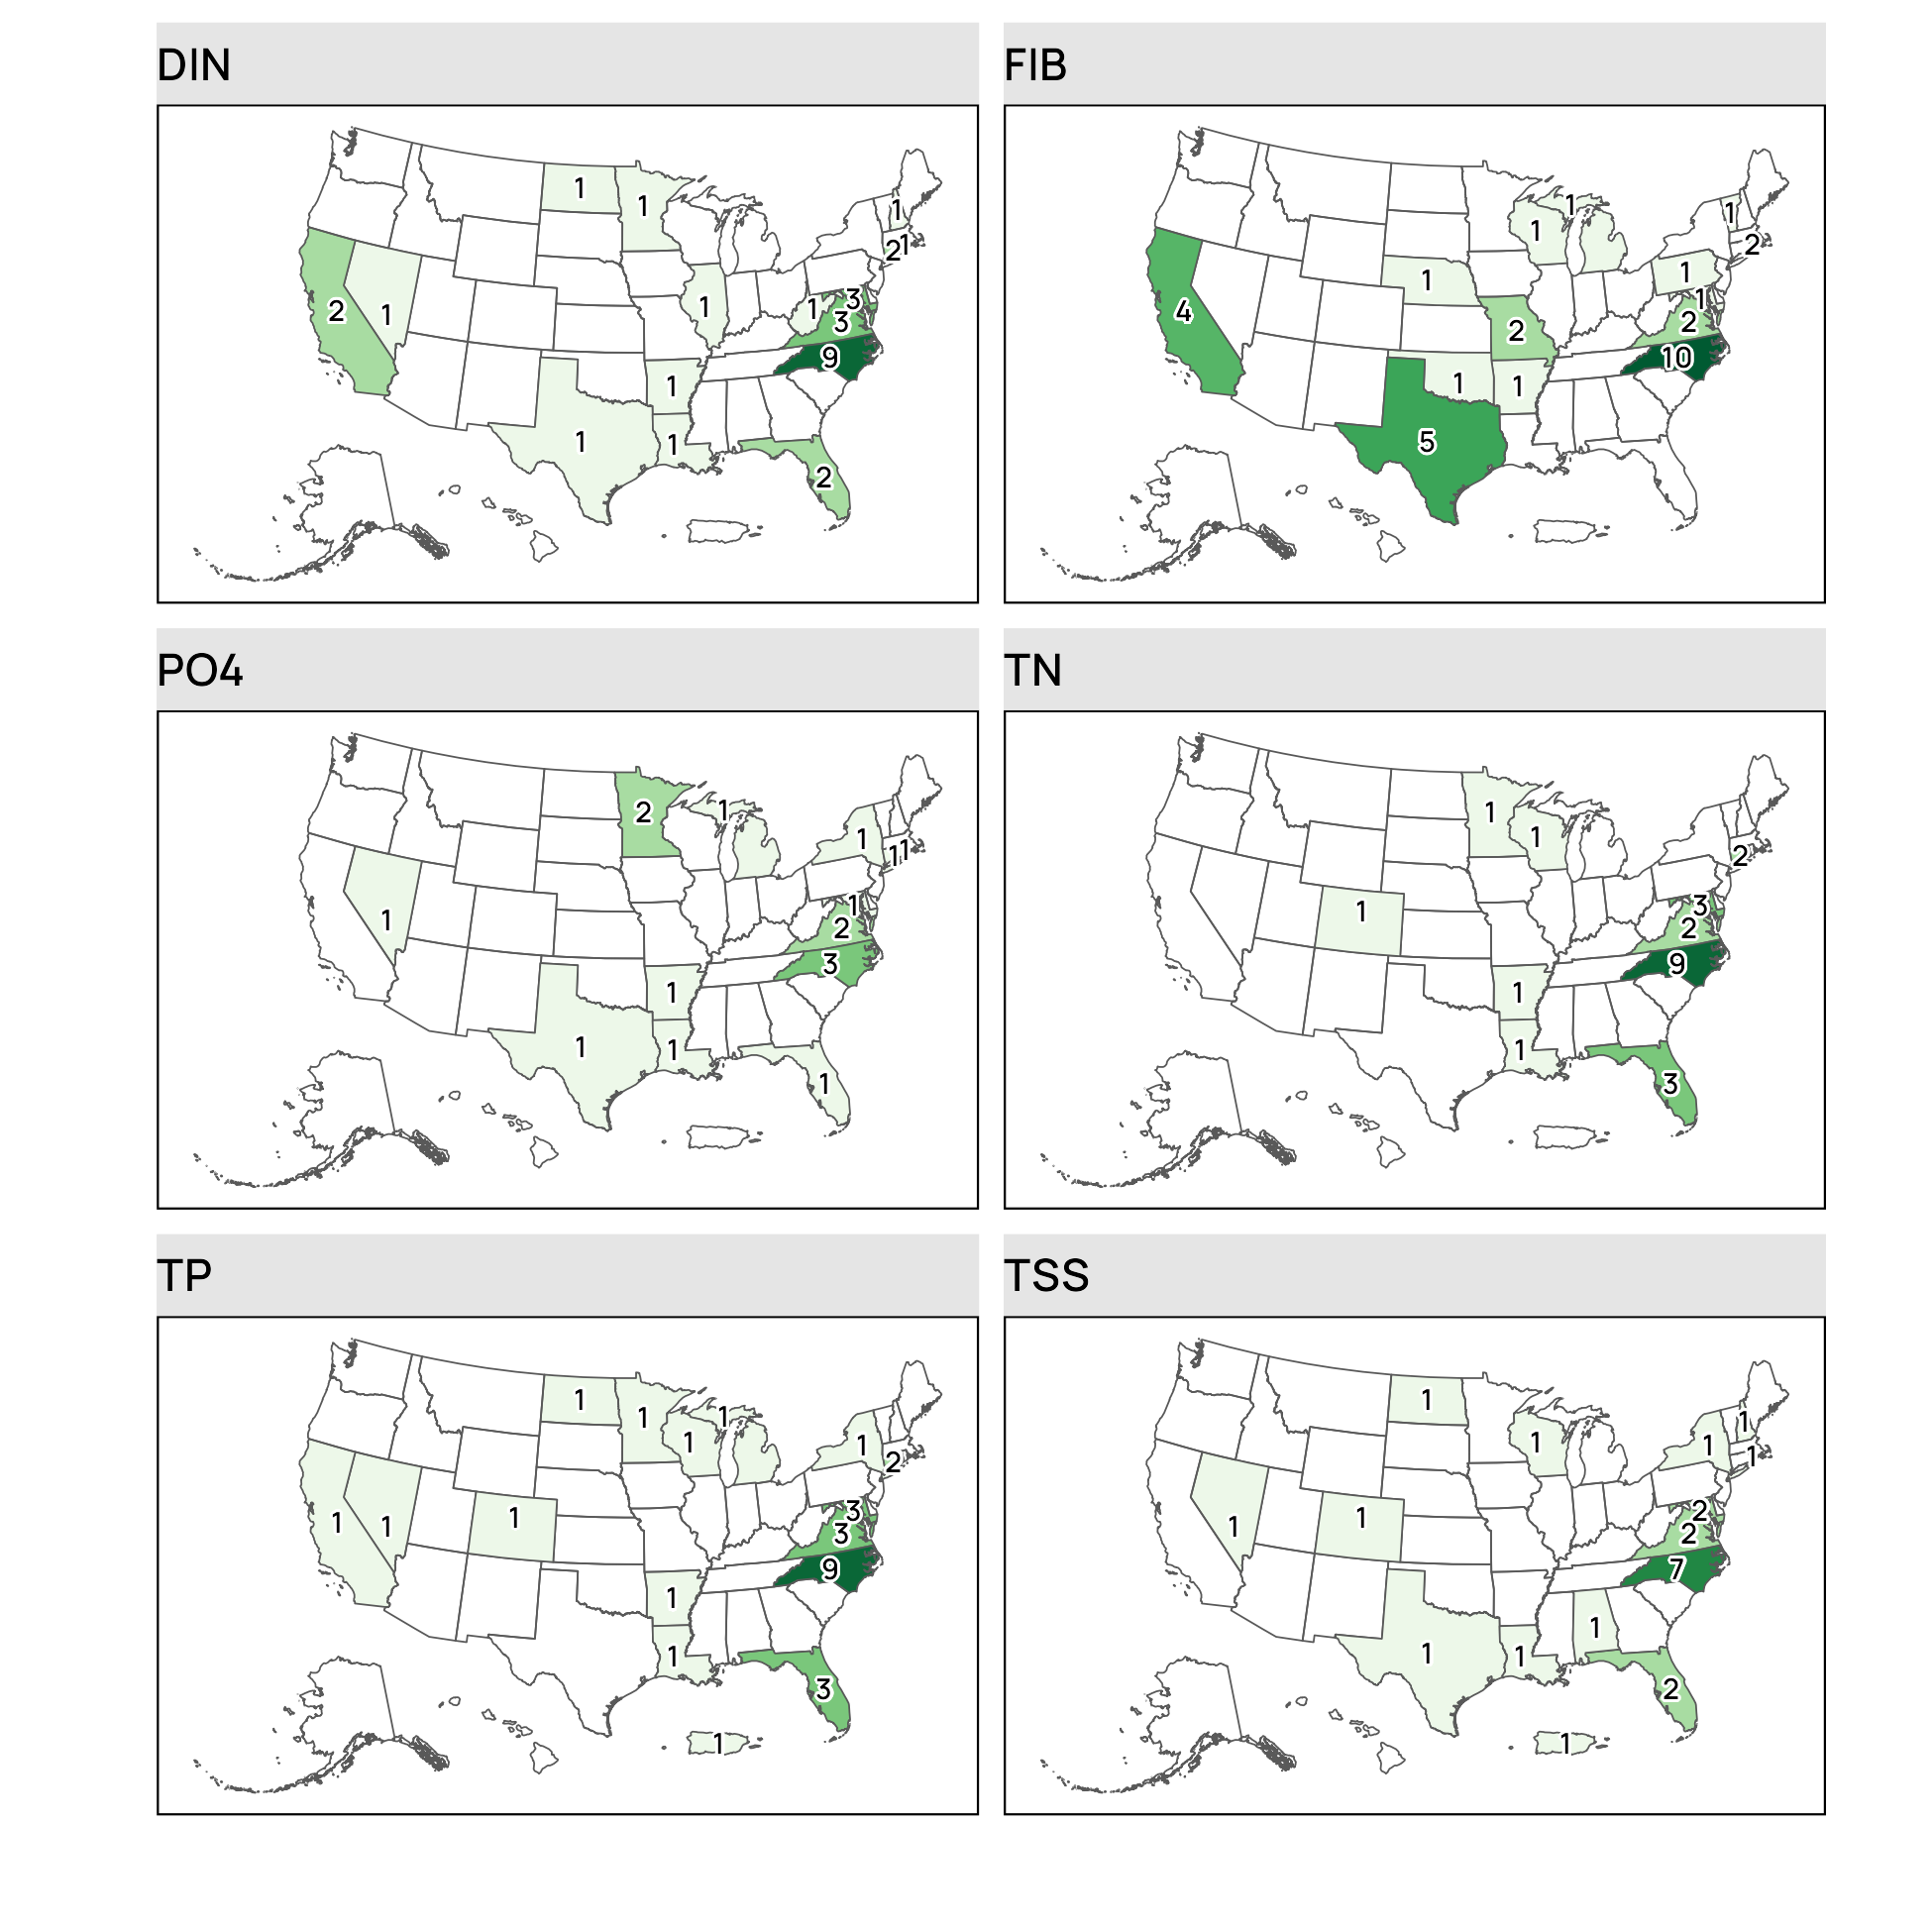
\includegraphics[width=0.5\textwidth,height=\textheight]{Schramm-UCOWR-2024_files/figure-beamer/p3-1.png}
\end{frame}

\begin{frame}{Results}
\phantomsection\label{results}
\begin{columns}[T]
\begin{column}{0.6\textwidth}
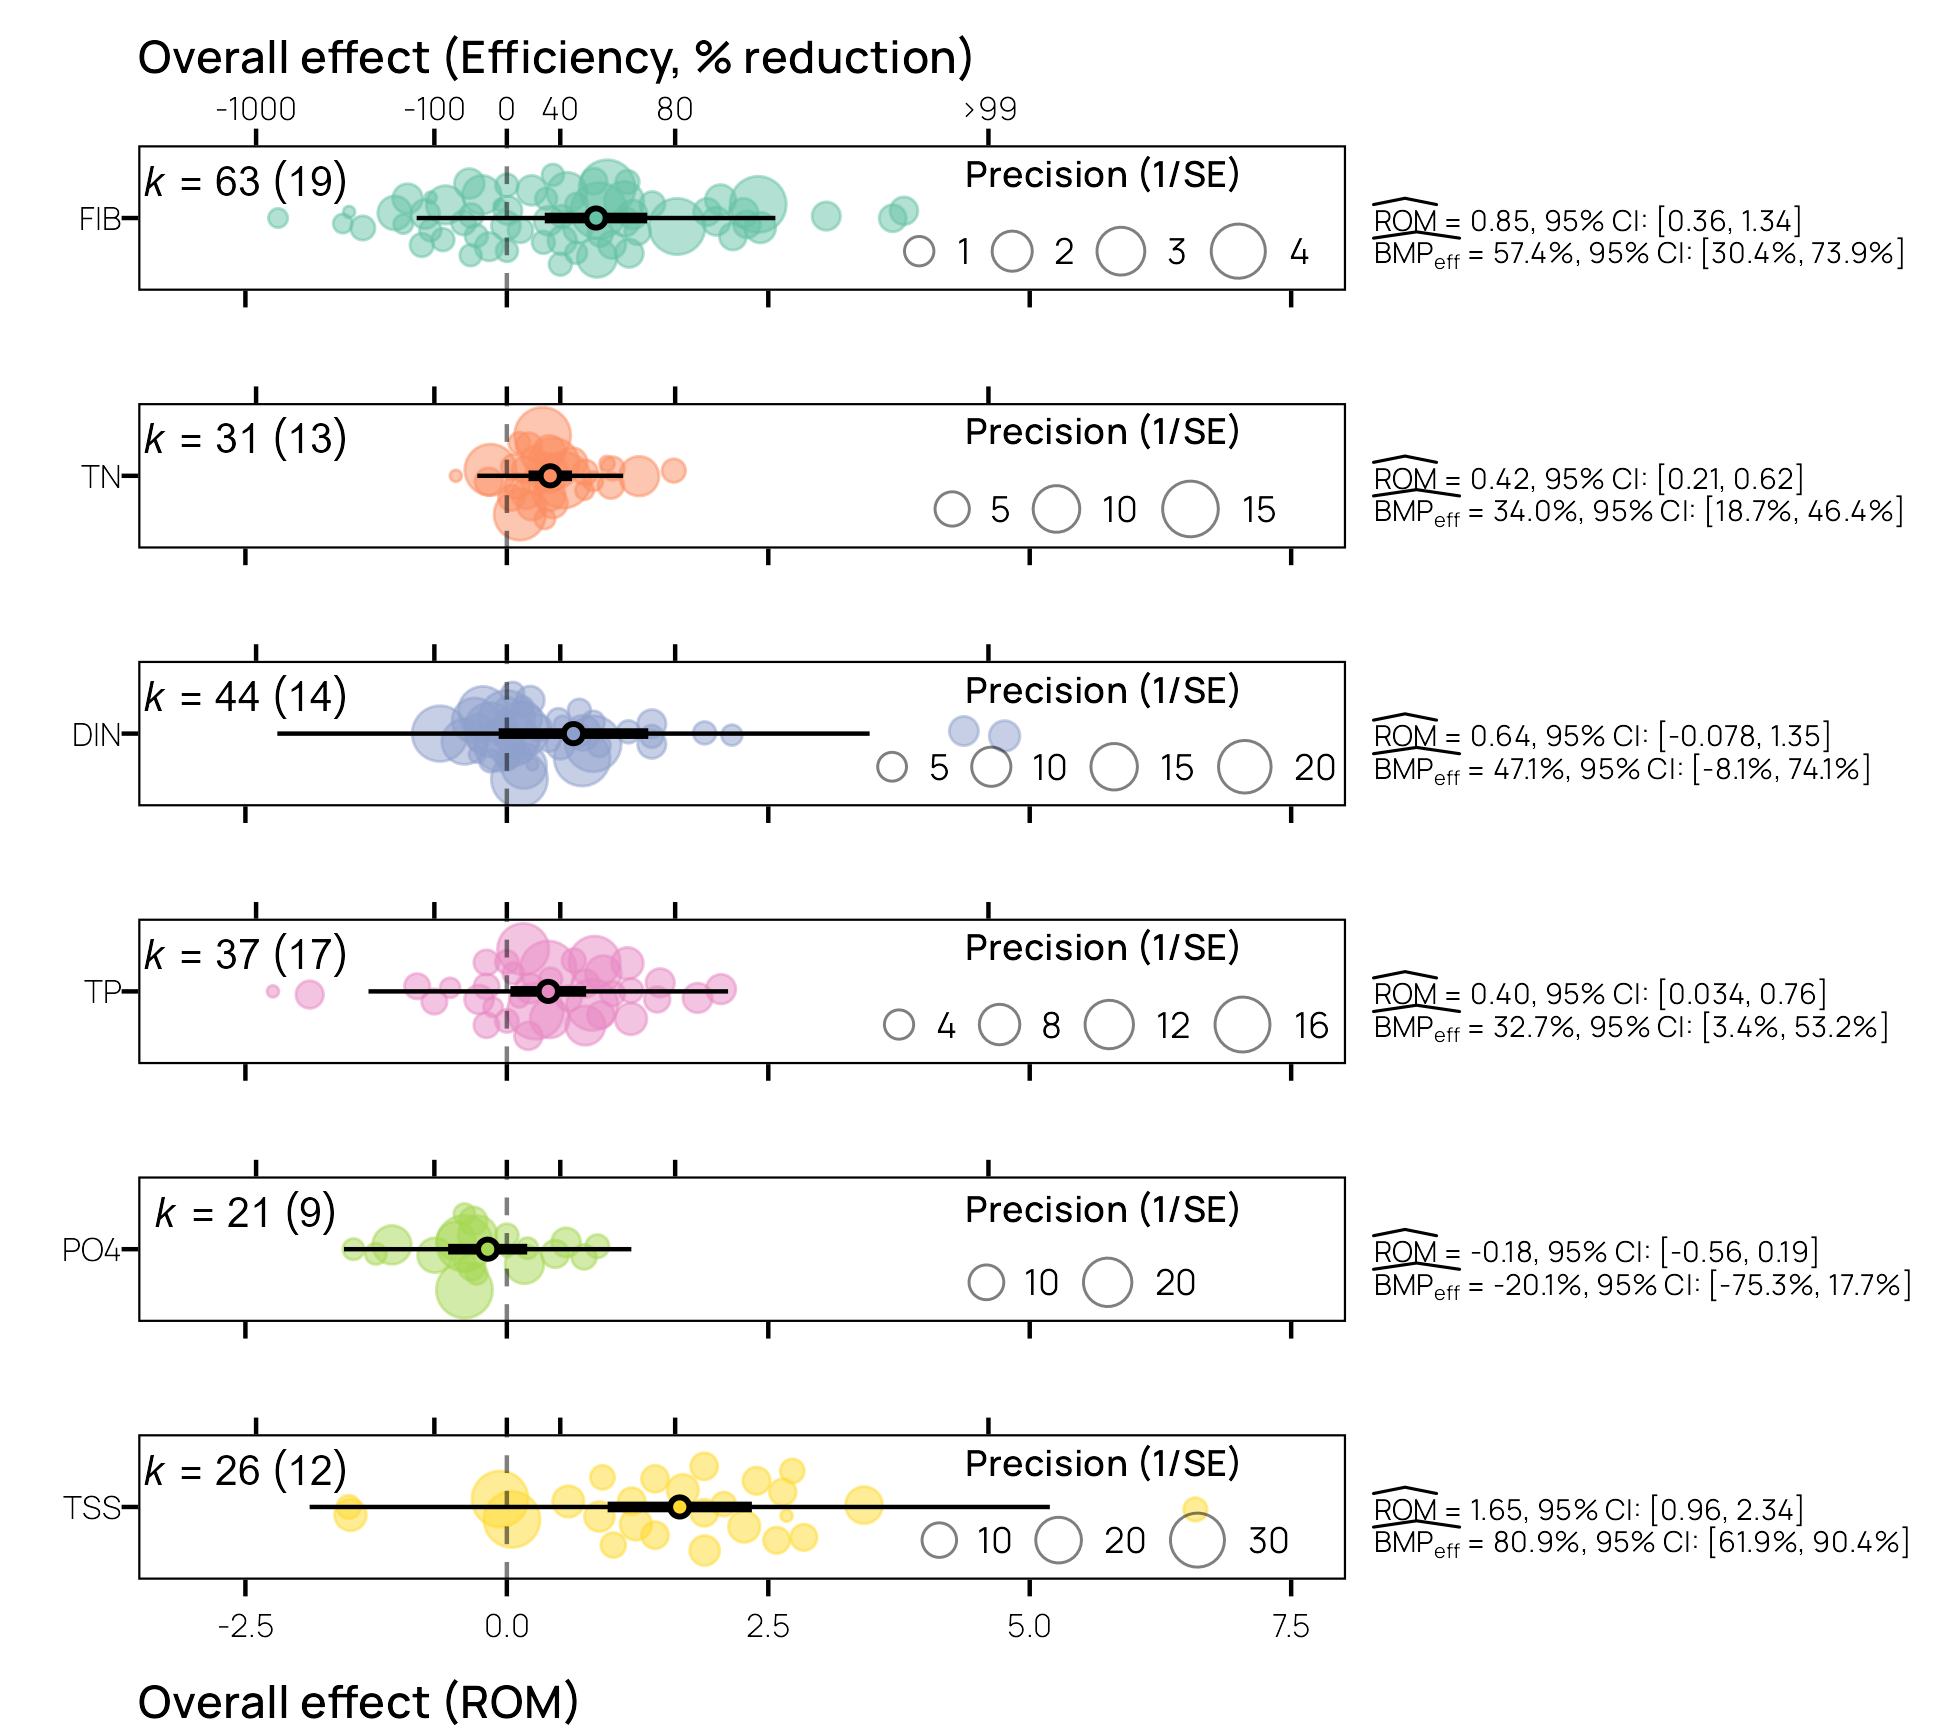
\includegraphics[width=1\textwidth,height=\textheight]{Schramm-UCOWR-2024_files/figure-beamer/p4-1.png}
\end{column}

\begin{column}{0.4\textwidth}
\begin{block}{Overall Effect}
\phantomsection\label{overall-effect}
\begin{itemize}
\tightlist
\item
  Strong evidence across studies for mean reductions in:

  \begin{itemize}
  \tightlist
  \item
    \textbf{FIB (57\%)}
  \item
    \textbf{TN (34\%)}
  \item
    \textbf{TP (32\%)}
  \item
    \textbf{TSS (81\%)}
  \end{itemize}
\item
  Prediction intervals provide low certainty about the performance of
  future \emph{individual} studies.
\end{itemize}
\end{block}
\end{column}
\end{columns}
\end{frame}

\begin{frame}{Attempts to Explain Variation in BMP Performance}
\phantomsection\label{attempts-to-explain-variation-in-bmp-performance}
\begin{columns}[T]
\begin{column}{0.4\textwidth}
\begin{tabular}[t]{l|l}
\hline
Parameter & Moderators\\
\hline
FIB & \makecell[l]{Influent Concentration,\\Aridity × BMP Subcategory}\\
\hline
TP & Influent Concentration\\
\hline
PO\textsubscript{4} & Influent Concentration\\
\hline
\end{tabular}

Influent concentration + Aridity×BMP Subcategory explained
\textasciitilde89\% of effect size variance in FIB models.
\end{column}

\begin{column}{0.6\textwidth}
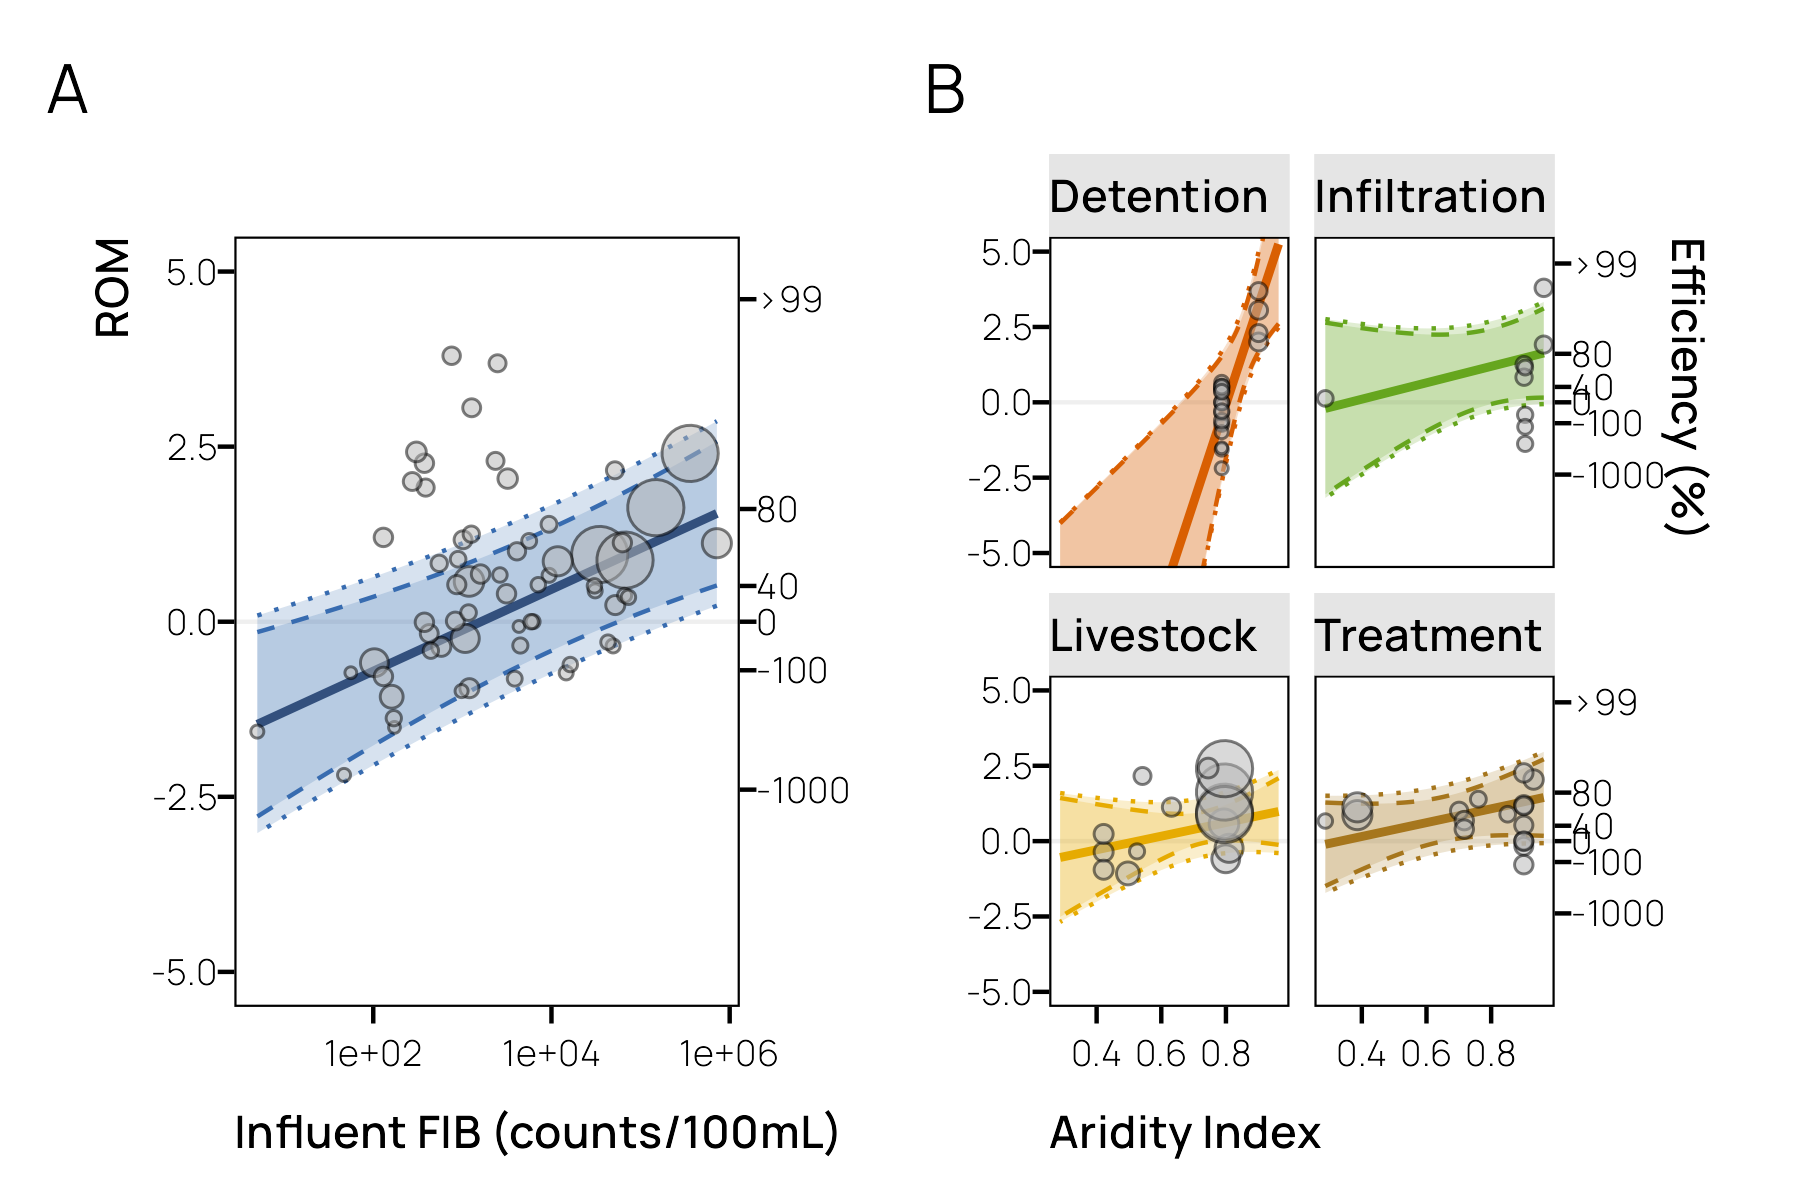
\includegraphics[width=1\textwidth,height=\textheight]{Schramm-UCOWR-2024_files/figure-beamer/p5-1.png}
\end{column}
\end{columns}
\end{frame}

\begin{frame}{Attempts to Explain Variation in BMP Performance}
\phantomsection\label{attempts-to-explain-variation-in-bmp-performance-1}
\begin{columns}[T]
\begin{column}{0.5\textwidth}
\begin{tabular}[t]{l|l}
\hline
Parameter & Moderators\\
\hline
FIB & \makecell[l]{Influent Concentration,\\Aridity × BMP Subcategory}\\
\hline
TP & Influent Concentration\\
\hline
PO\textsubscript{4} & Influent Concentration\\
\hline
\end{tabular}

Influent concentration explained 12\% and 35\% of effect size variance
in TP and PO\textsubscript{4} models.
\end{column}

\begin{column}{0.5\textwidth}
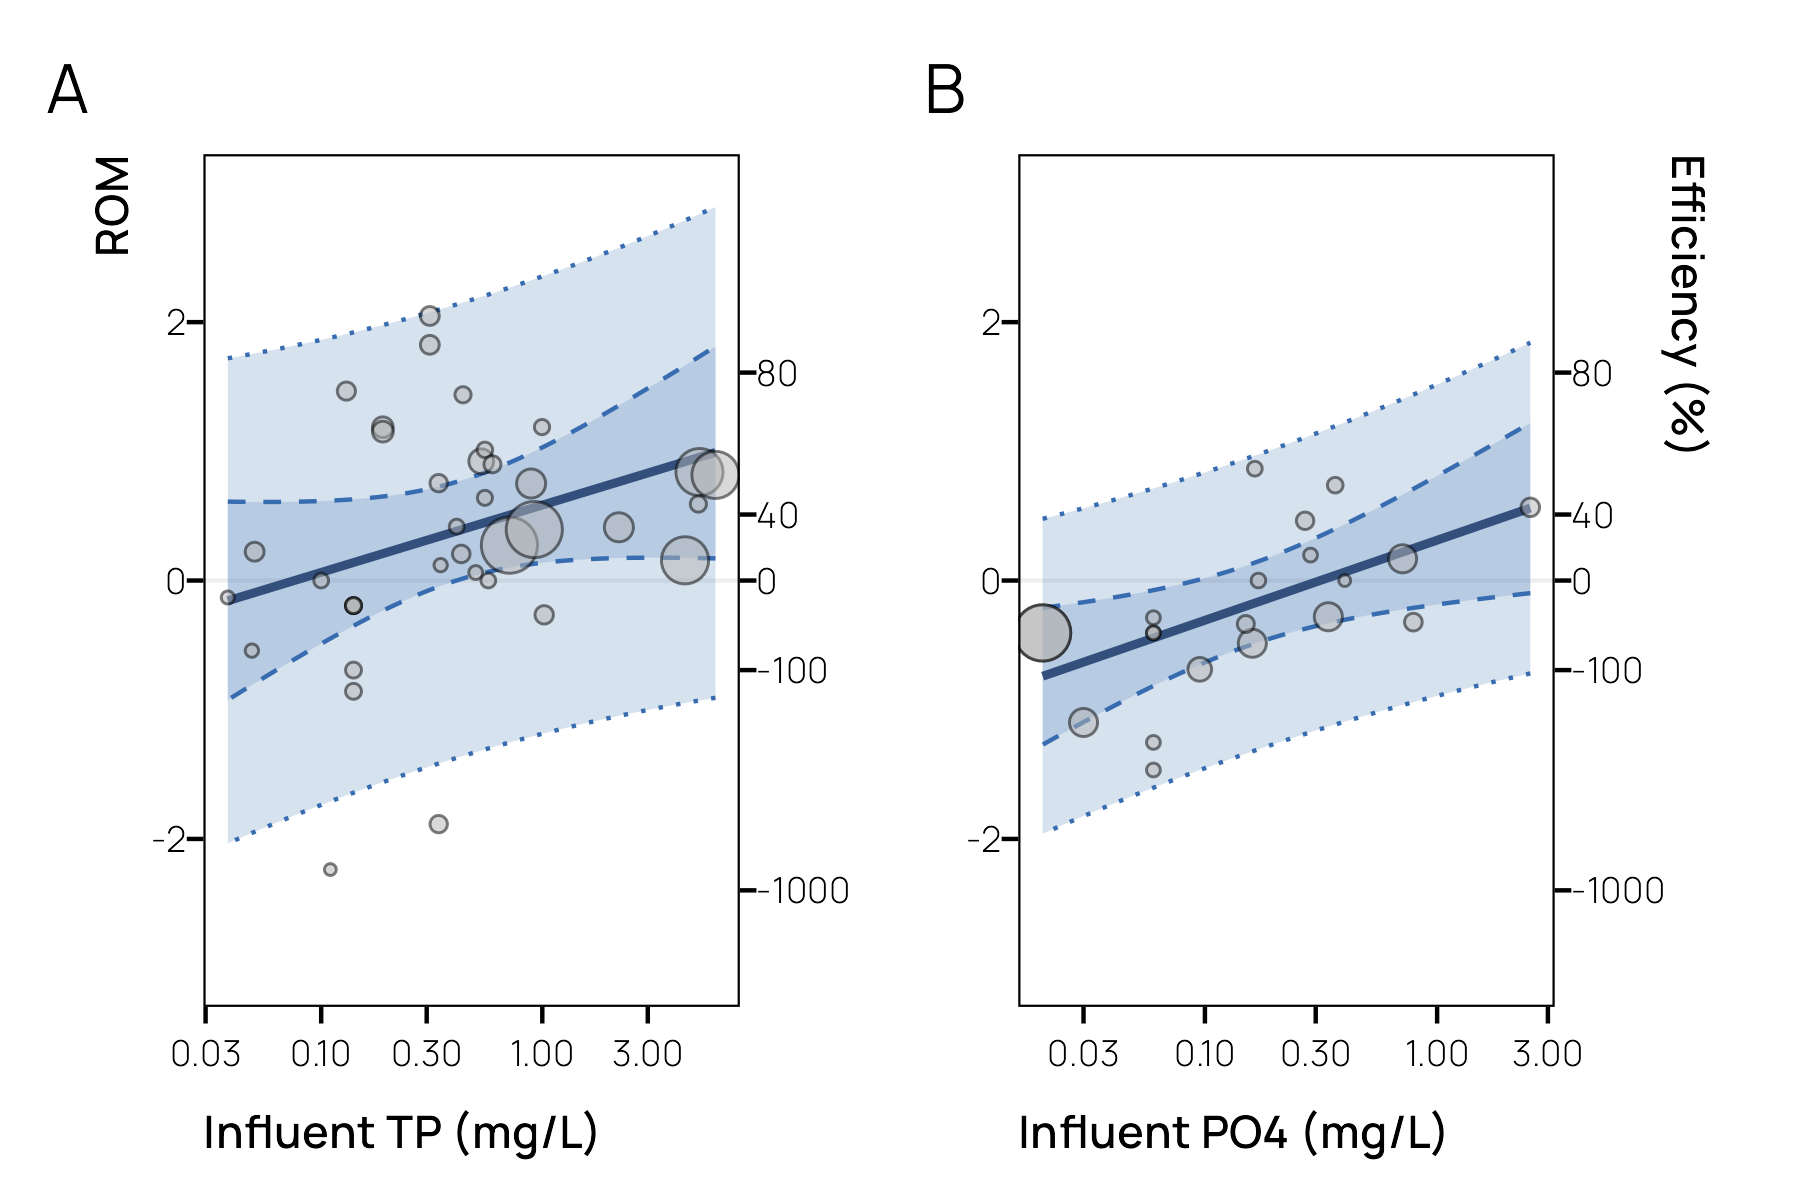
\includegraphics[width=1\textwidth,height=\textheight]{Schramm-UCOWR-2024_files/figure-beamer/p6-1.png}
\end{column}
\end{columns}
\end{frame}

\begin{frame}{Overview}
\phantomsection\label{overview}
\begin{itemize}
\tightlist
\item
  Few long-term studies (\textgreater4 year).
\item
  Studies clustered in the mid-Atlantic, low spatial variability.
\item
  Studies demonstrated mean reductions in FIB, TN, TP, and TSS.
\item
  Did not find evidence for mean reductions in DIN, PO\textsubscript{4}.
\item
  Influent concentration has strong influence on FIB, TP, and
  PO\textsubscript{4} performance.
\item
  Failed to explain majority of variance in nutrient and TSS models.
  \textbf{(Why???)}
\end{itemize}
\end{frame}

\begin{frame}{Lessons Learned}
\phantomsection\label{lessons-learned}
\textbf{Issues in Published BMP Studies}

\begin{itemize}
\tightlist
\item
  Very inconsistent reporting of non-manipulated study conditions.
\item
  Earlier studies tended to report BMP efficiency only.
\item
  Many studies fail to report sample size, variance, or uncertainty
  measures (59\% of identified effect sizes).
\item
  There is an opportunity to develop reporting protocols for BMP
  studies. See Eagle et
  al.~\footfullcite{eagleMetaAnalysisConstrained2017}

  \begin{itemize}
  \tightlist
  \item
    Environmental variables, reported metrics, regression model
    reporting\ldots{}
  \end{itemize}
\end{itemize}
\end{frame}

\begin{frame}{Lessons Learned}
\phantomsection\label{lessons-learned-1}
\textbf{Study/Systematic Review Issues}

\begin{itemize}
\tightlist
\item
  Broad study design (focus on specific BMP types).
\item
  Keyword comprehensiveness.
\item
  \emph{metafor} R package facilitates
  meta-analysis.\footfullcite{viechtbauerConductingMetaanalysesMetafor2010}
\item
  Developing and training students/staff on data extraction is
  difficult.
\item
  Data entry interfaces that reinforce data consistency.
\end{itemize}
\end{frame}

\begin{frame}{Thank You}
\phantomsection\label{thank-you}
\textbf{Contact:} michael.schramm@ag.tamu.edu

\textbf{Acknowledgements:} Texas State Soil and Water Conservation Board
for funding.

\textbf{Paper:} Schramm M, Kikoyo D, Wright J and Jain S (2024) A
meta-analysis of the impacts of best management practices on nonpoint
source pollutant concentration. Front. Water 6:1397615. doi:
10.3389/frwa.2024.1397615

\textbf{Data:} Kikoyo D, Jain S, Wright J, and Schramm M. (2024). TWRI
NPS-BMP-DB (v1.05). Zenodo. doi: 10.5281/zenodo.10451303
\end{frame}


%\begin{frame}[allowframebreaks]{}
%  \bibliographytrue
%  %\printbibliography[heading=none]
%\end{frame}



\end{document}
